\begin{figure}[]
	\centering
	\begin{subfigure}{.45\textwidth}
		\centering
		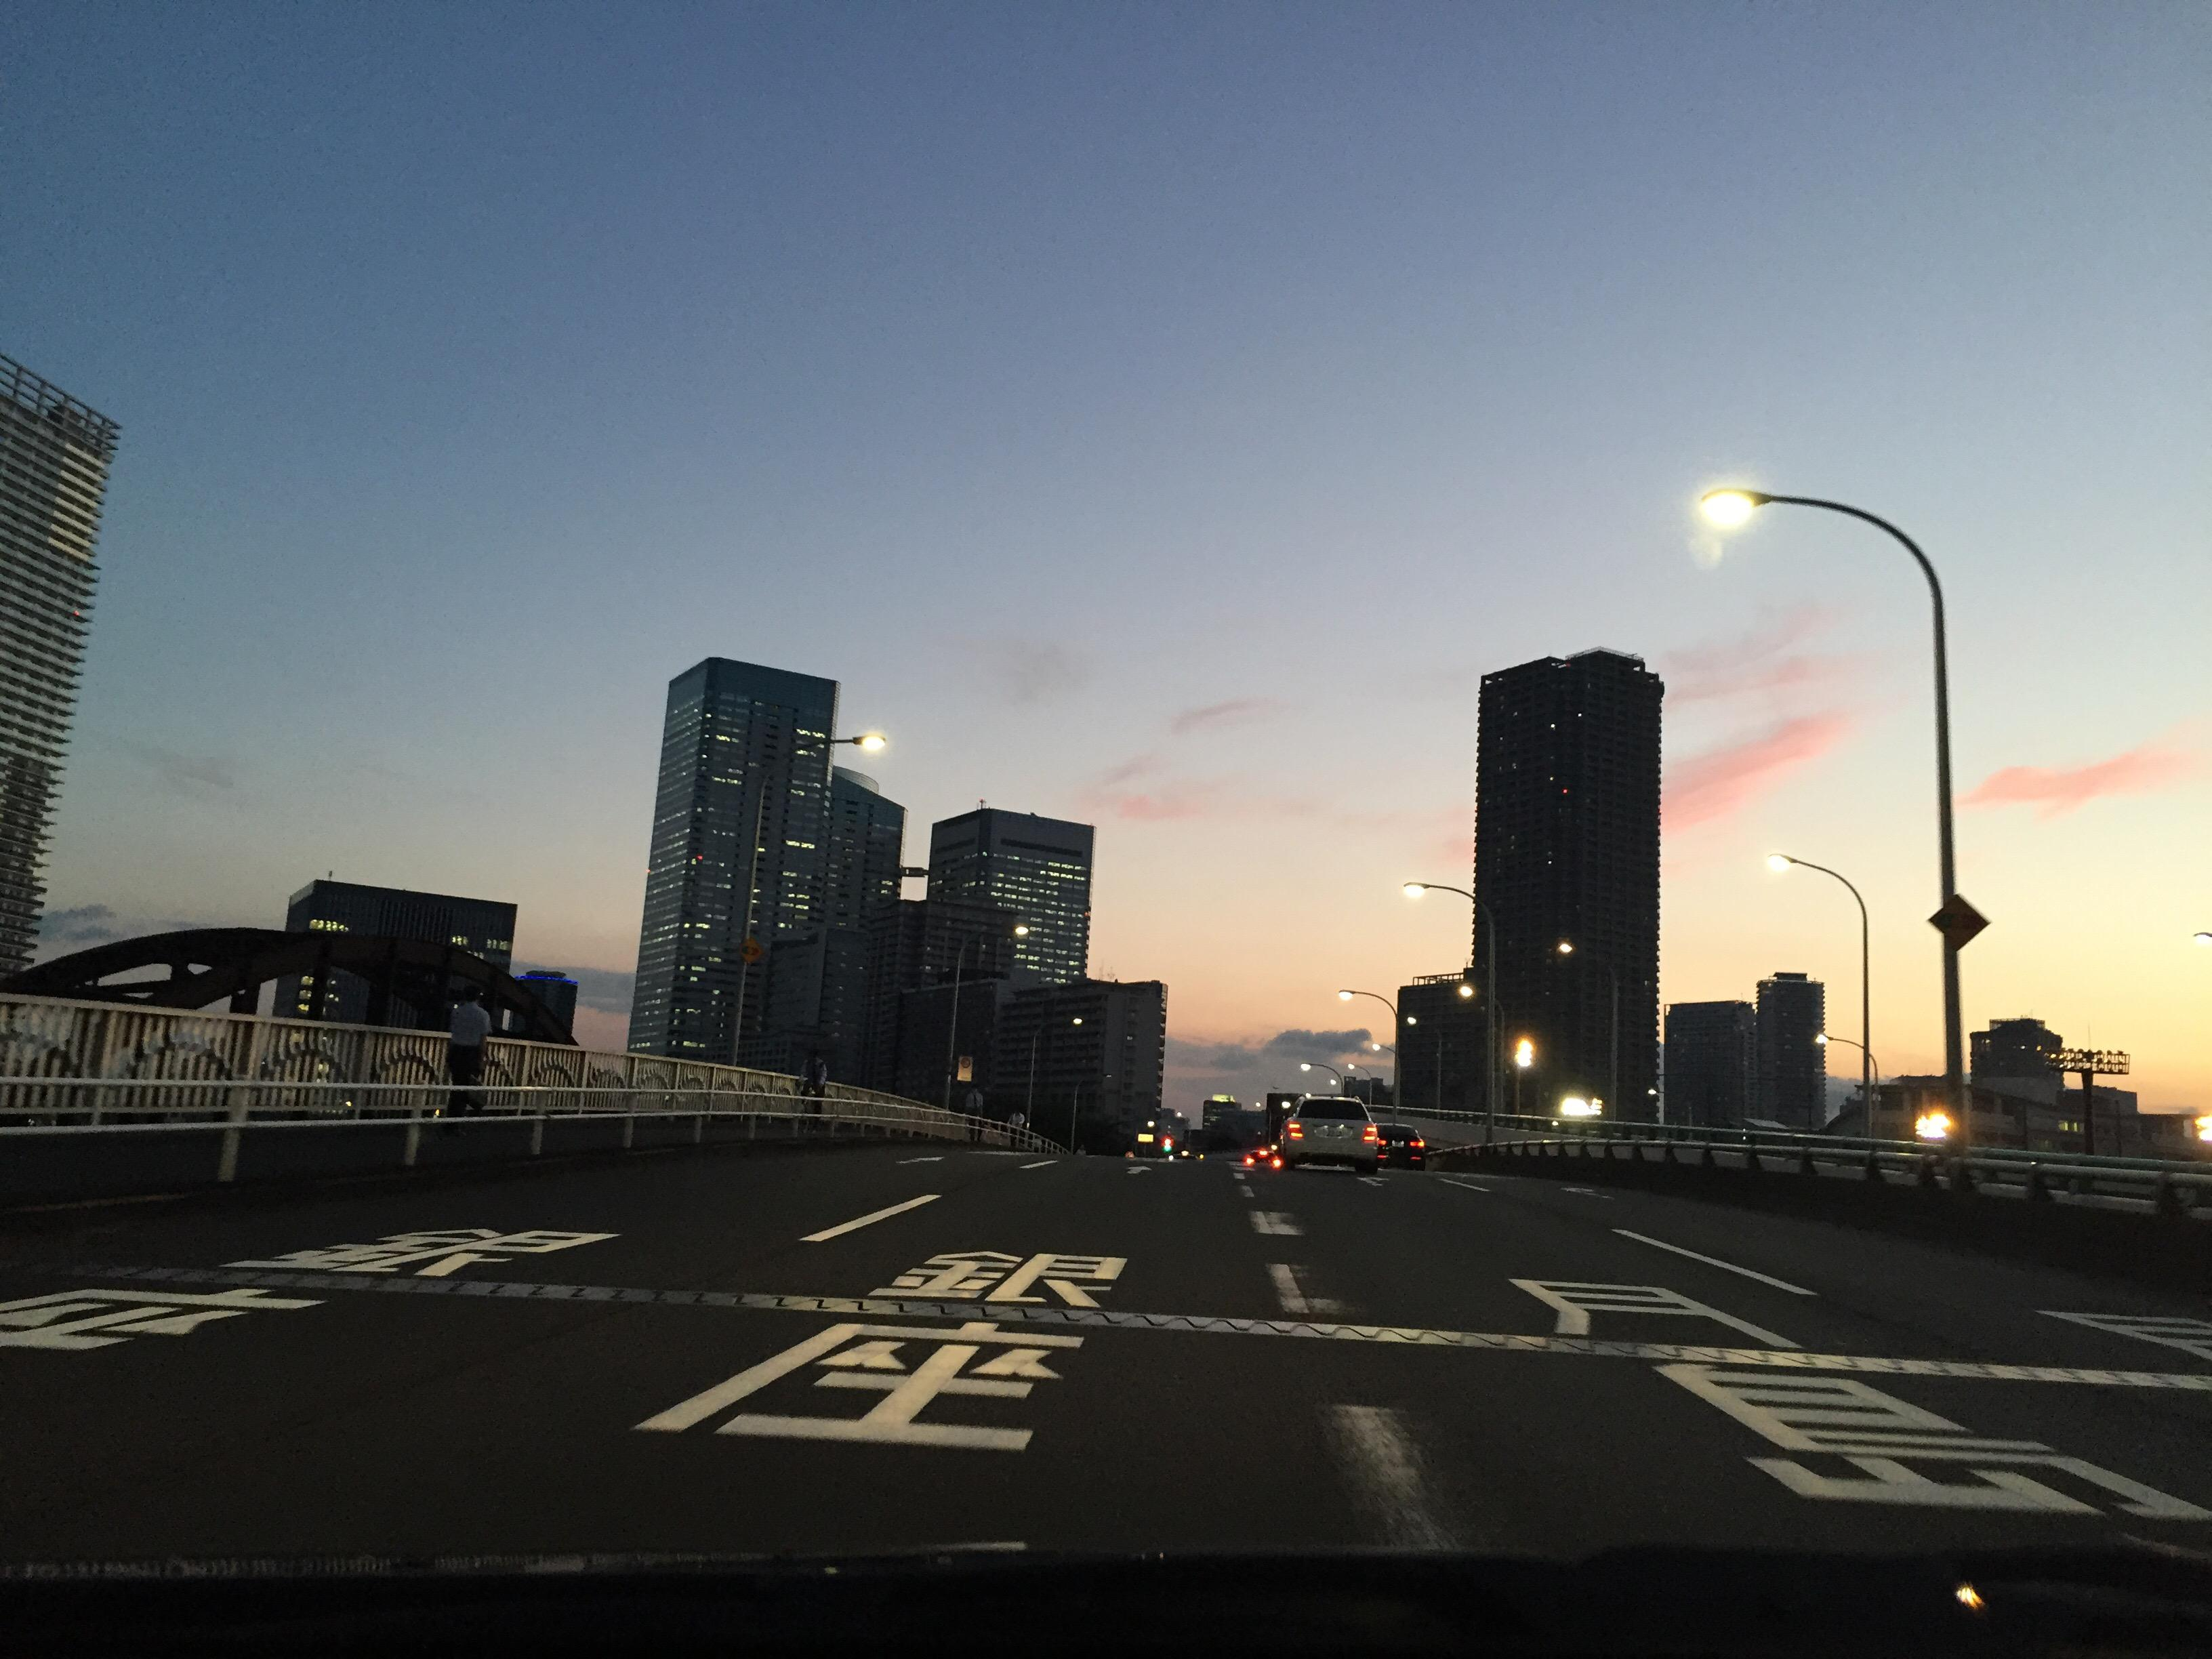
\includegraphics[width=\linewidth]{figures/experiments/dataset/1.jpg}
		\caption[Dataset Sample 1]{This image shows an axample of an evening scene.}
		\label{fig:dataset-1}
	\end{subfigure}
	\hfill
	\begin{subfigure}{.45\textwidth}
		\centering
		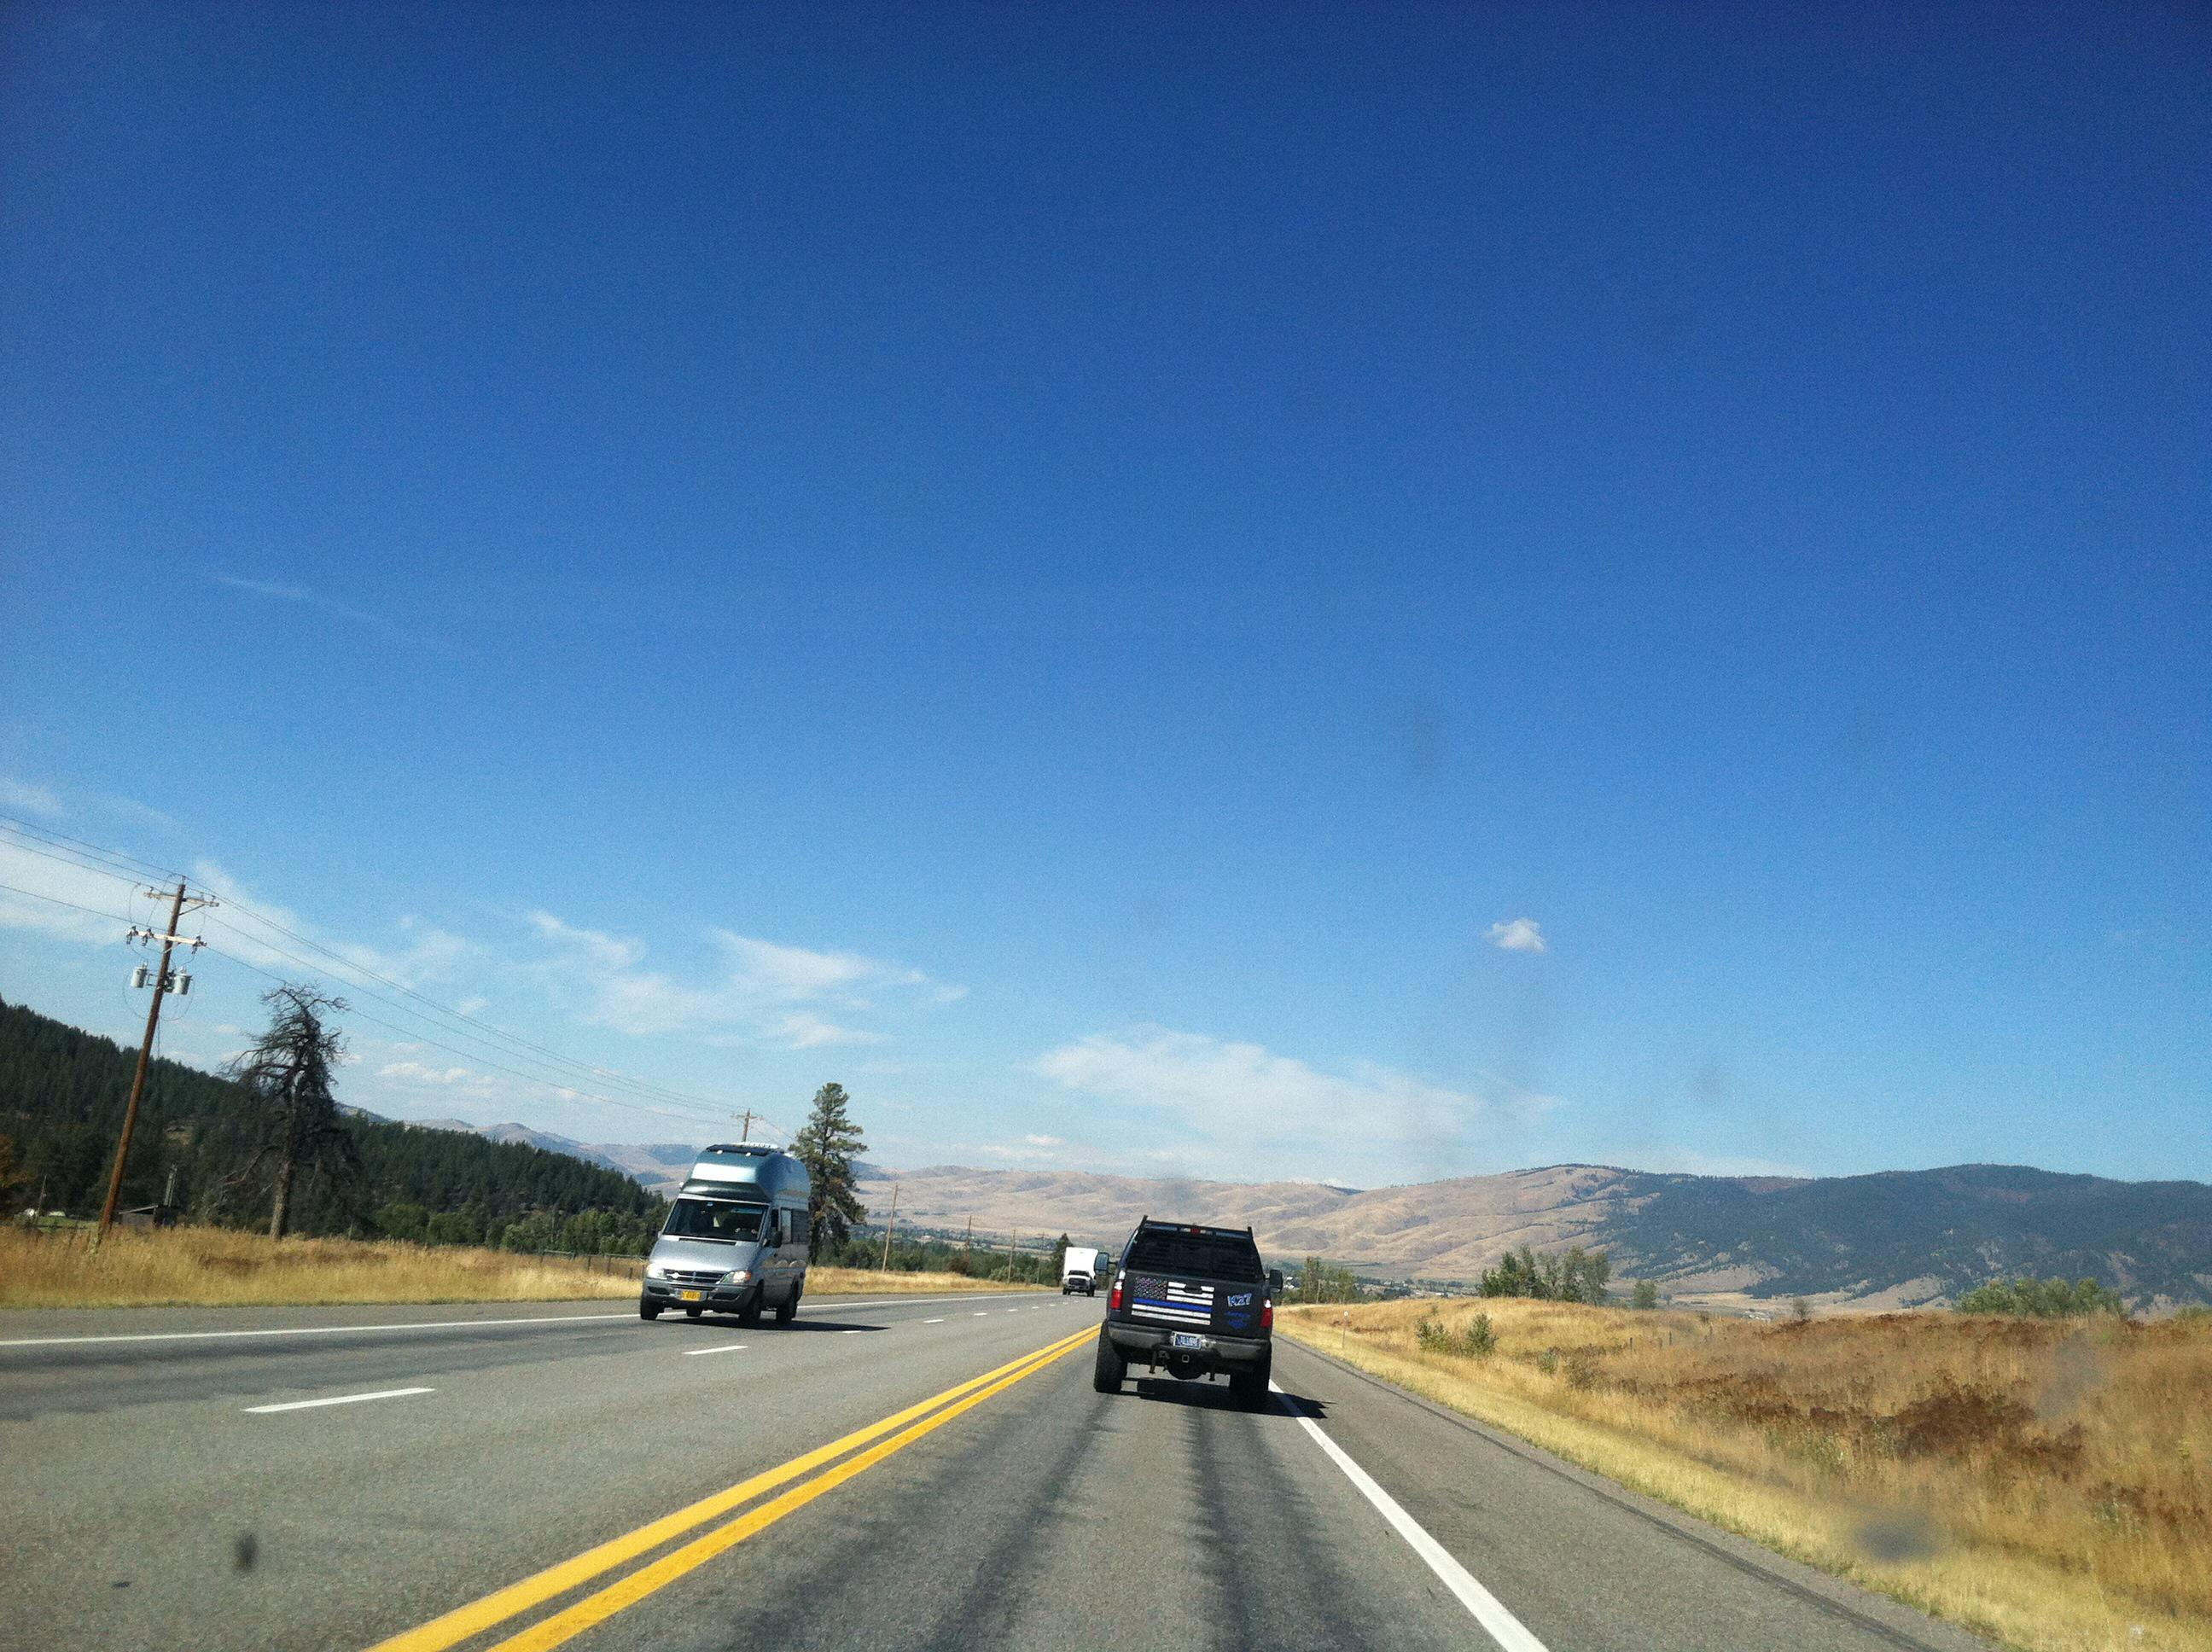
\includegraphics[width=\linewidth]{figures/experiments/dataset/2.jpg}
		\caption[Dataset Sample 2]{This image shows an example of a very bright scene in a rural area.}
		\label{fig:dataset-2}
	\end{subfigure}
	
	\vspace{12pt}%------------ 
	
	\begin{subfigure}{.45\textwidth}
		\centering
		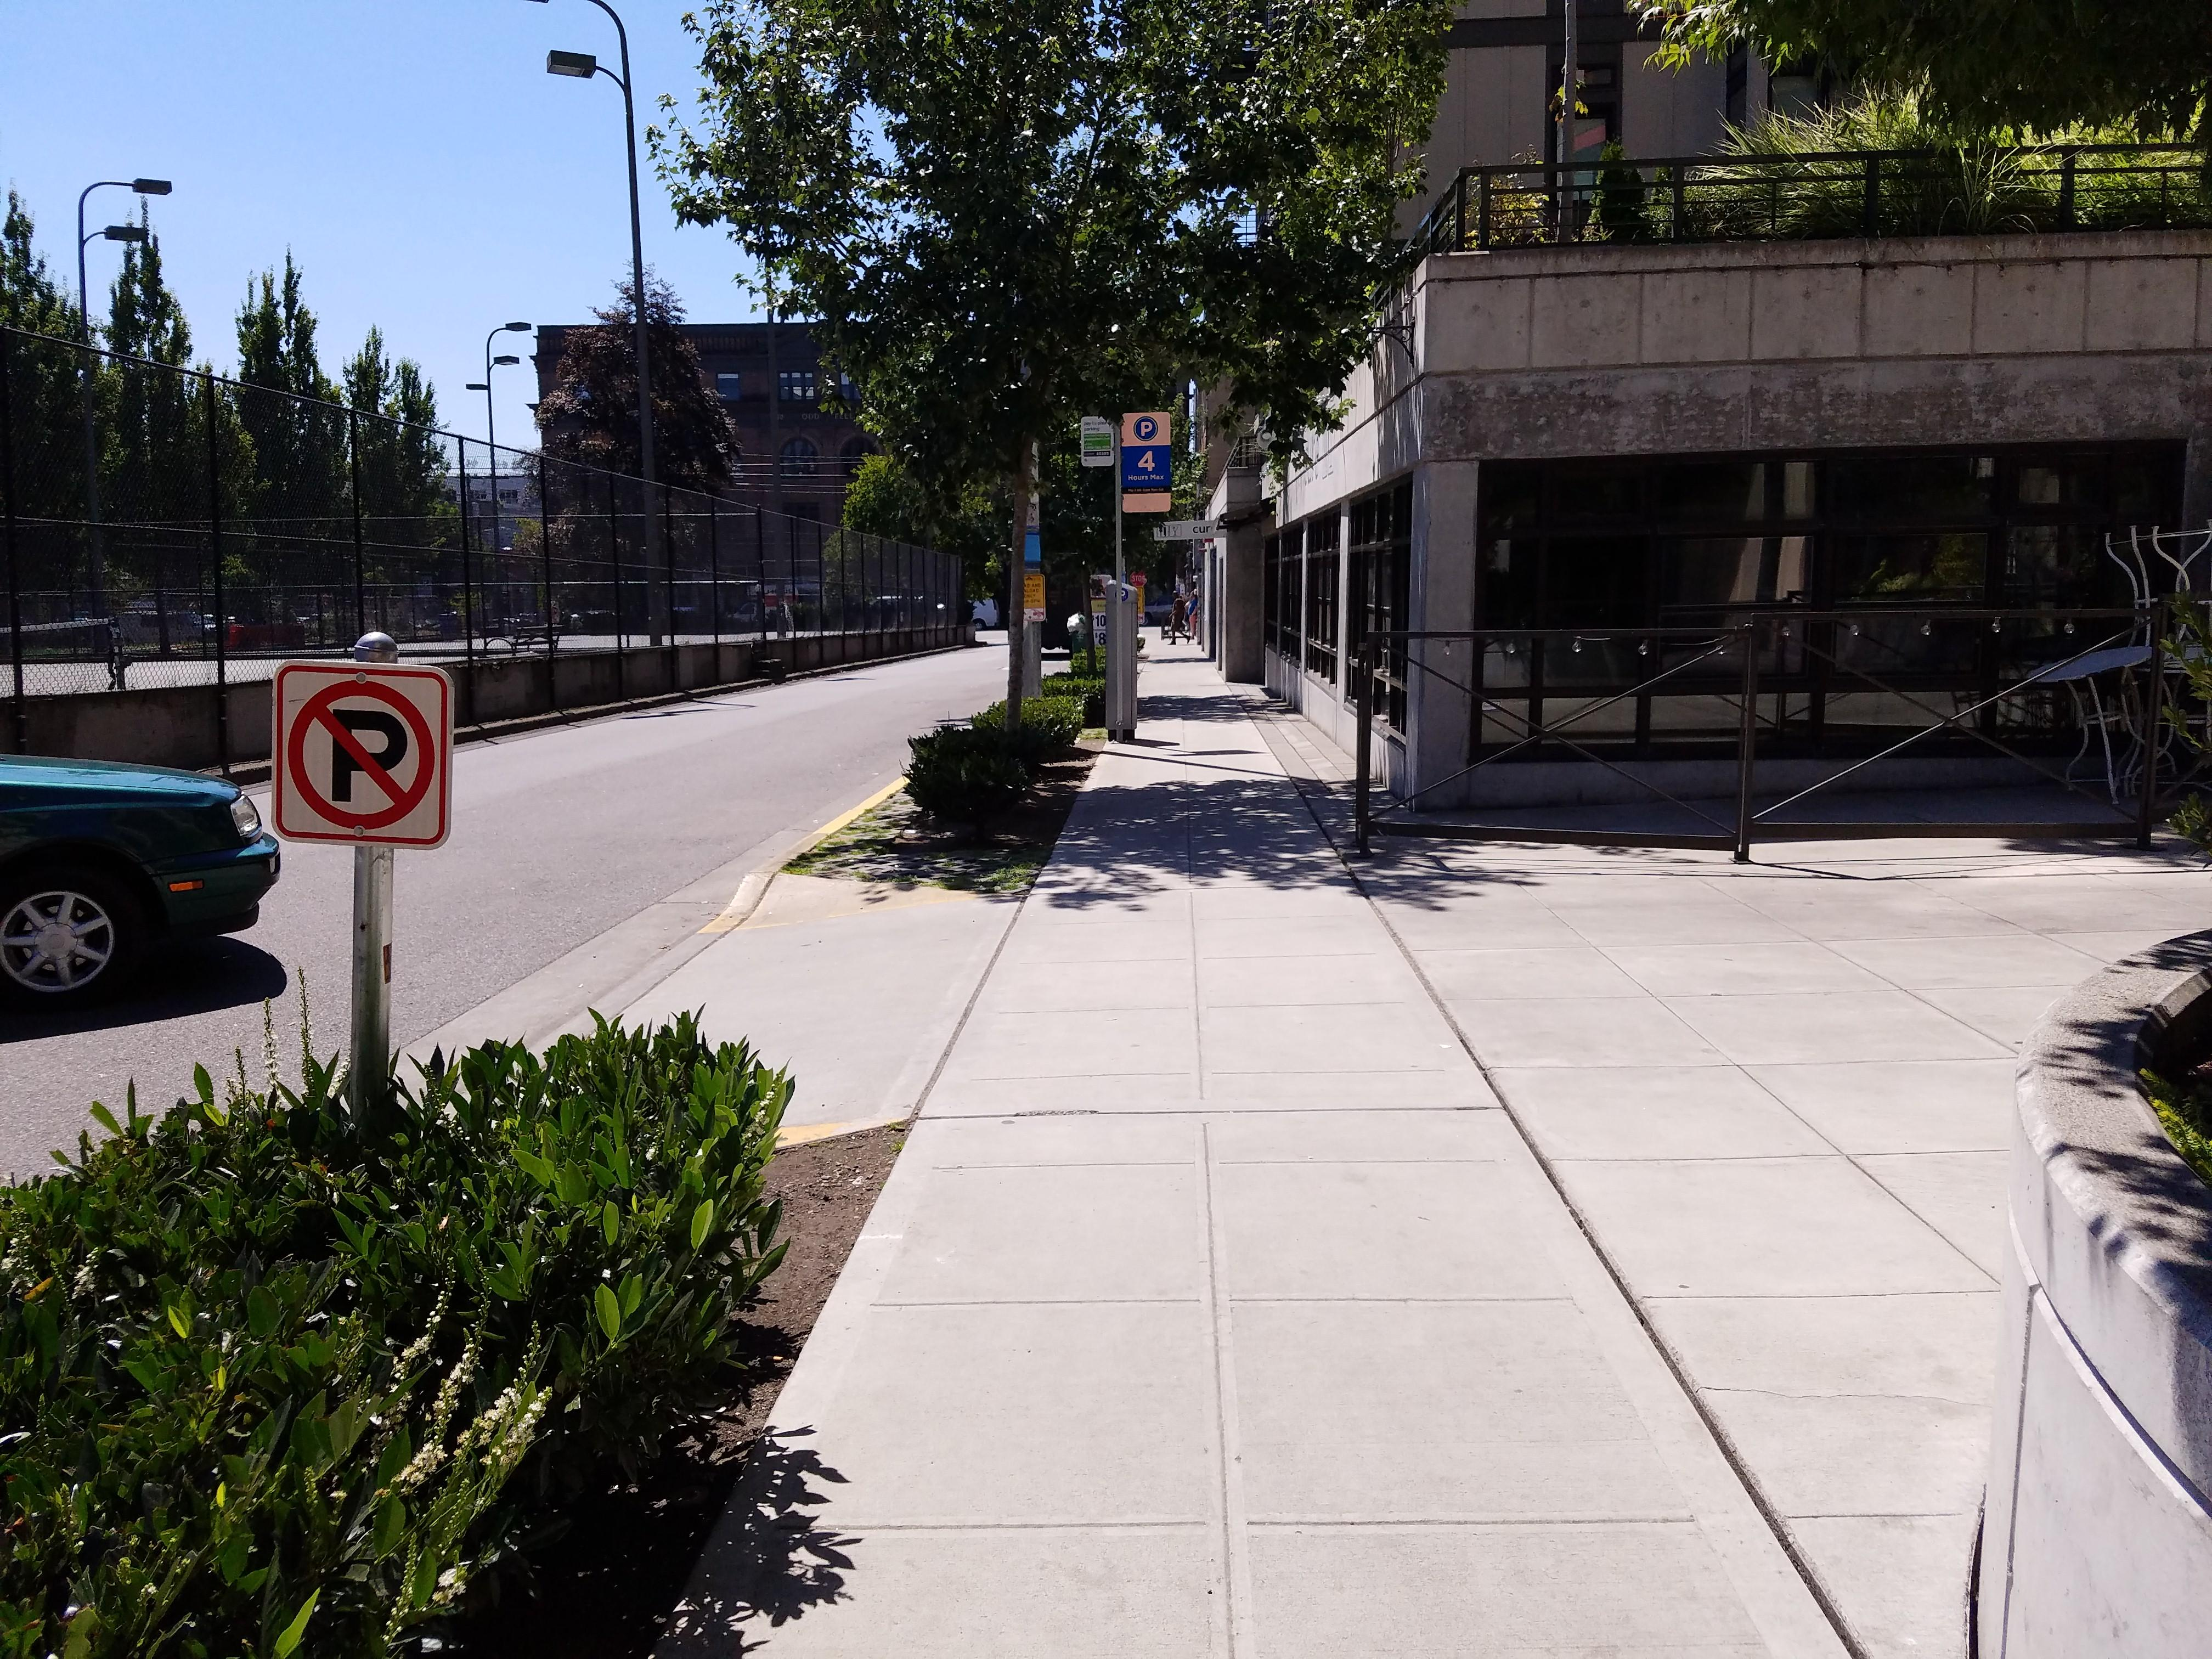
\includegraphics[width=\linewidth]{figures/experiments/dataset/3.jpg}
		\caption[Dataset Sample 3]{This image shows an example of an image from a sidewalk.}
		\label{fig:dataset-3}
	\end{subfigure}
	\hfill
	\begin{subfigure}{.45\textwidth}
		\centering
		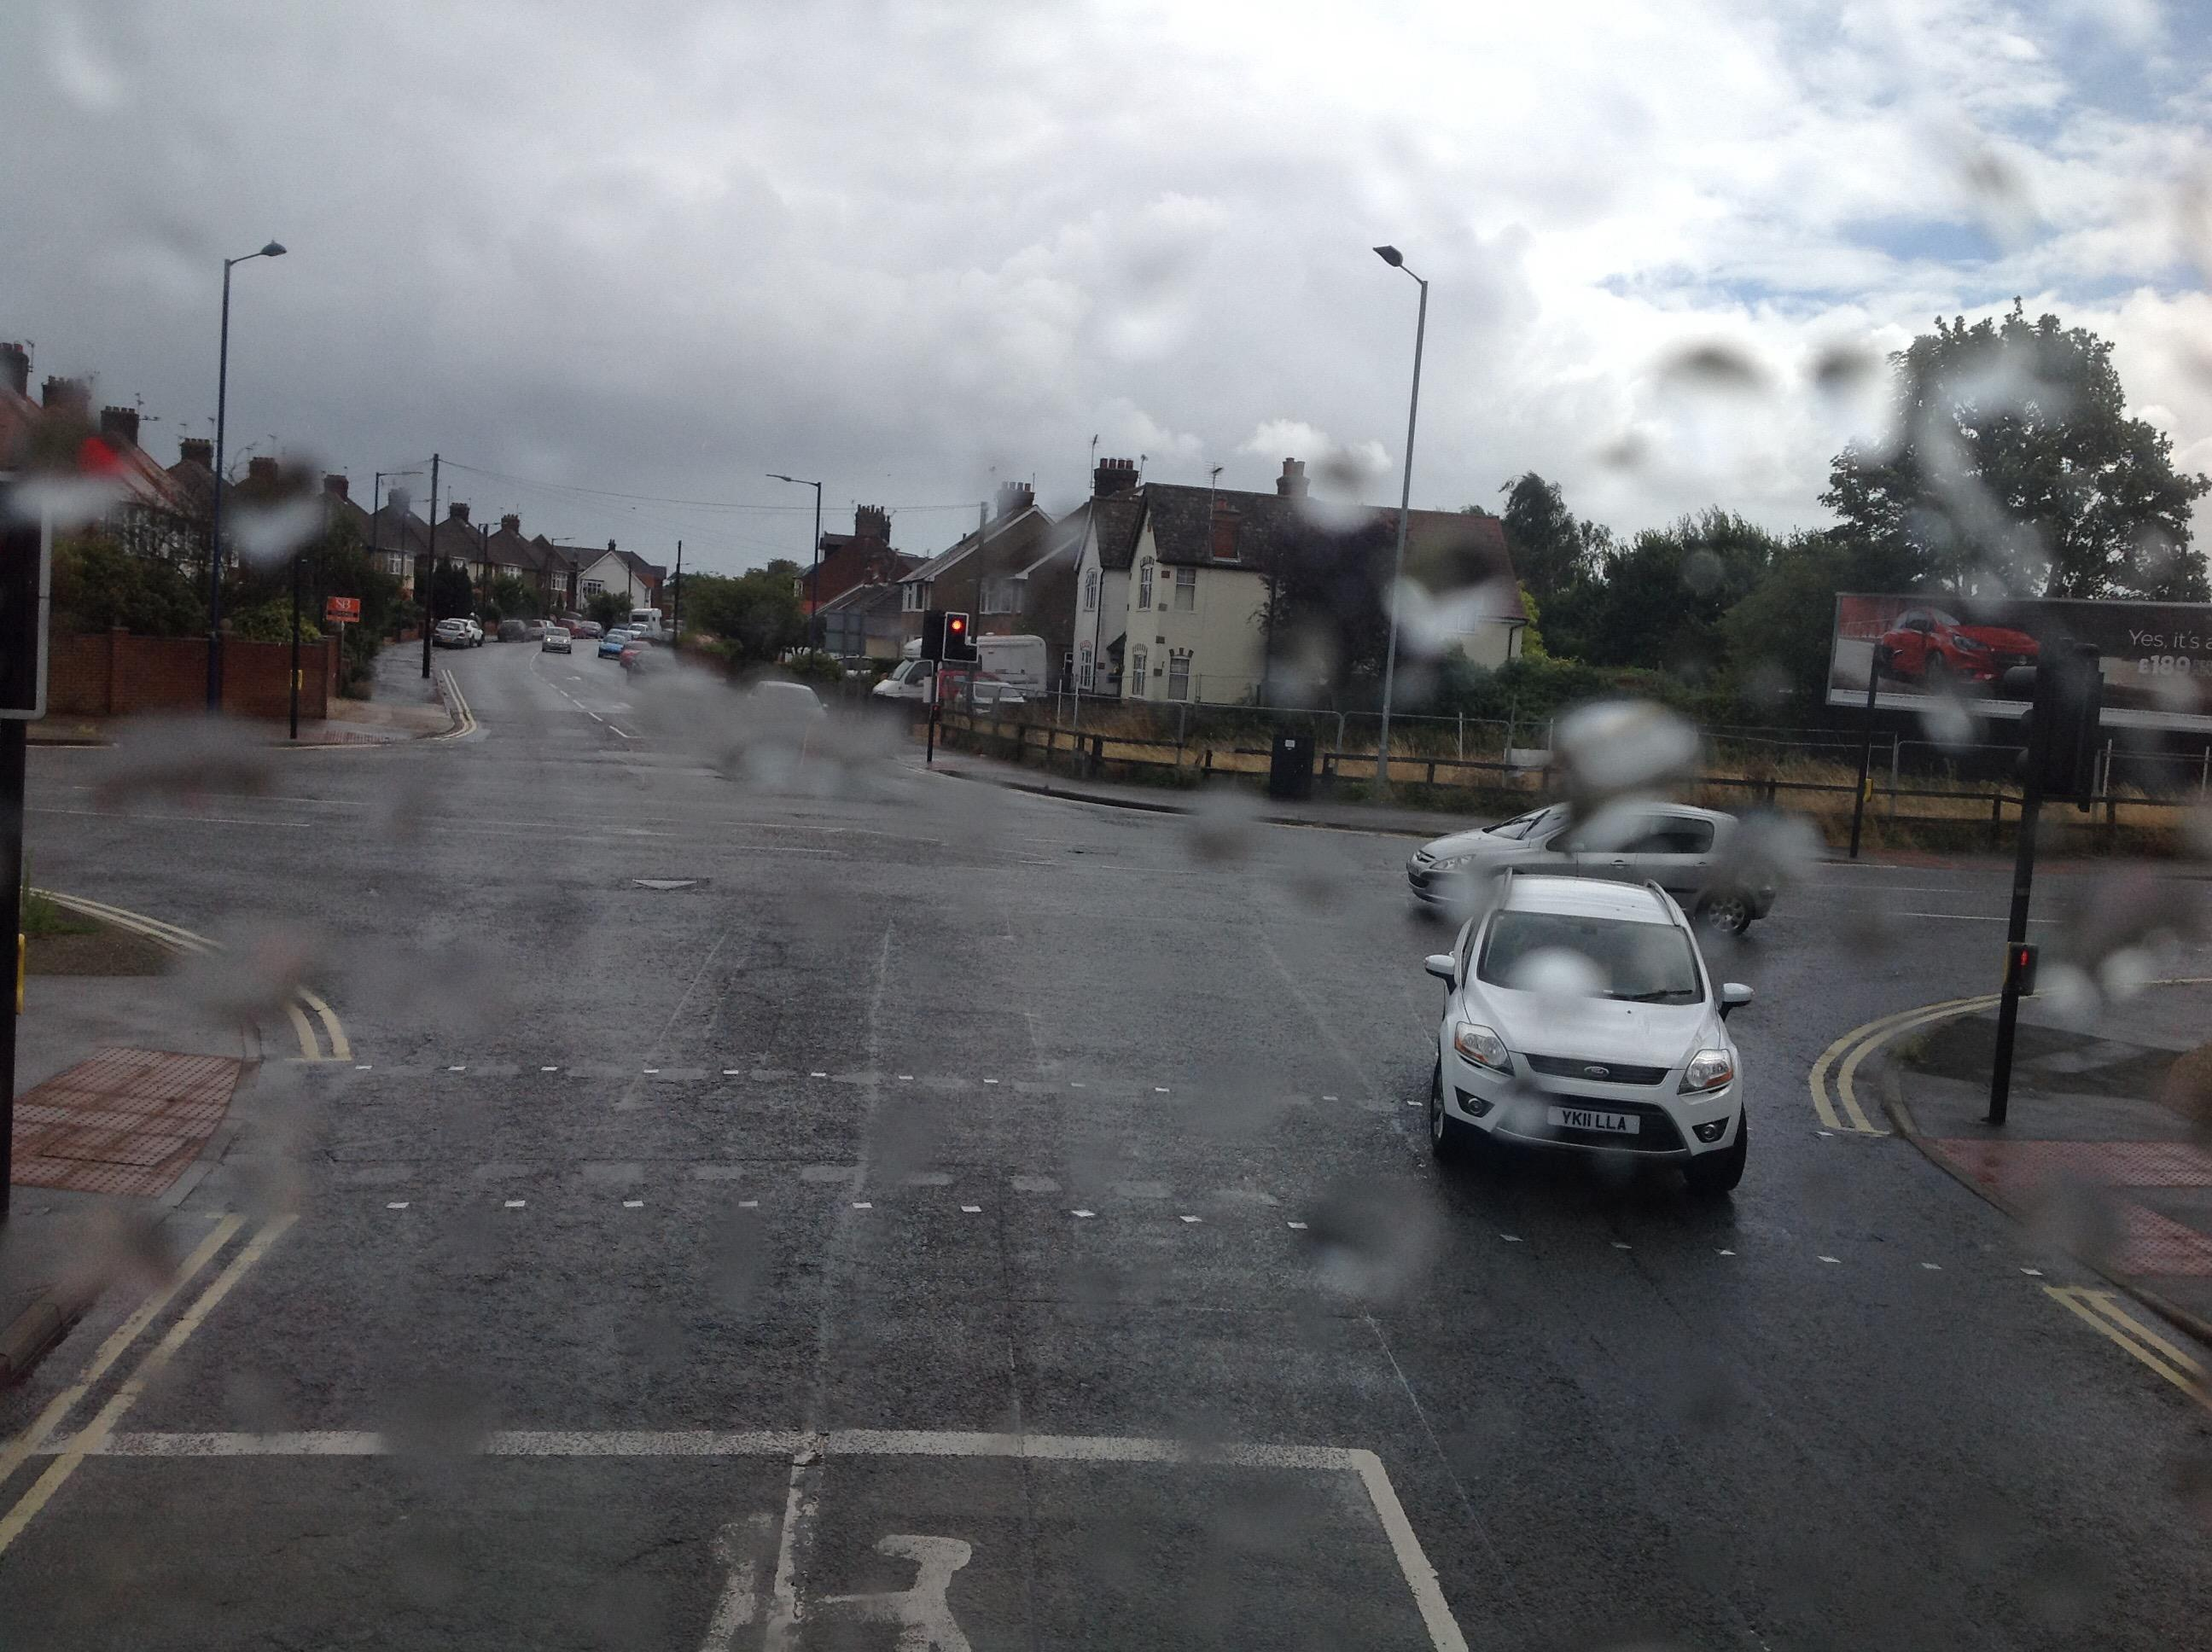
\includegraphics[width=\linewidth]{figures/experiments/dataset/4.jpg}
		\caption[Dataset Sample 4]{This image shows an example of an image taken during rainy conditions.}
		\label{fig:dataset-4}
	\end{subfigure}

	\caption[Mapillary Vistas Dataset Sample Images]{These sample images from the Mapillary dataset shows how varied and diverse the dataset is. This diversity makes the dataset an excellent choice in training a network that can generalize to unseen conditions.}
	\label{fig:experiments-datasetsamples}
\end{figure}